\documentclass[10pt, table, dvipsnames,xcdraw, handout]{beamer}
\usetheme[progressbar=frametitle]{metropolis}
\usepackage{appendixnumberbeamer}
\usetikzlibrary{arrows.meta, positioning, quotes}
\usepackage[shortlabels]{enumitem}
\usepackage{xcolor}
\usepackage{mathtools}
\usepackage{dsfont}

\usepackage{caption}


\usepackage{cancel}

\newcommand\hcancel[2][black]{\setbox0=\hbox{$#2$}%
\rlap{\raisebox{.45\ht0}{\textcolor{#1}{\rule{\wd0}{1pt}}}}#2} 


\usepackage{booktabs}
\usepackage[scale=2]{ccicons}

\usepackage{pgfplots}
\usepgfplotslibrary{dateplot}

\usepackage{xspace}
\newcommand{\themename}{\textbf{\textsc{metropolis}}\xspace}
\newcommand{\cb}{\cellcolor{blue!25}}


% Notation:
\newcommand{\cT}{\ensuremath{\mathcal{T}}}
\newcommand{\cD}{\ensuremath{\mathcal{D}}}
\newcommand{\cX}{\ensuremath{\mathcal{X}}}
\newcommand{\cY}{\ensuremath{\mathcal{Y}}}
\newcommand{\cZ}{\ensuremath{\mathcal{Z}}}
\newcommand{\cH}{\ensuremath{\mathcal{H}}}
\newcommand{\cG}{\ensuremath{\mathcal{G}}}

\newcommand{\bR}{\ensuremath{\mathbb{R}}}
\newcommand{\bN}{\ensuremath{\mathbb{N}}}
\newcommand{\bP}{\ensuremath{\mathbb{P}}}
\newcommand{\bT}{\ensuremath{\mathbb{T}}}
\newcommand{\bL}{\ensuremath{\mathbb{L}}}

\newcommand{\bfX}{\ensuremath{\mathbf{X}}}
\newcommand{\bfY}{\ensuremath{\mathbf{Y}}}
\newcommand{\bfy}{\ensuremath{\mathbf{y}}}
\newcommand{\bfD}{\ensuremath{\mathbf{D}}}

\def\layersep{2.5cm}

% Tikz seys
\tikzset{cross/.style={cross out, draw, 
         minimum size=2*(#1-\pgflinewidth), 
         inner sep=0pt, outer sep=0pt}}

\title{Machine Learning I}
\subtitle{Lecture 16: Cluster Analysis Part II}
% \date{\today}
\date{}
\author{Nathaniel Bade}
\institute{Northeastern University Department of Mathematics}
% \titlegraphic{\hfill\includegraphics[height=1.5cm]{logo.pdf}}

\begin{document}

\maketitle

\begin{frame}{Table of contents}
  \setbeamertemplate{section in toc}[sections numbered]
  \tableofcontents[hideallsubsections]
\end{frame}


%%%%%%%%%%%%%% Slidshow Start %%%%%%%%%%%%%% 


%Notes: 4 kinds of clusering: Centroid based/kmeans, connecctivity based, density based, distribution based. 
%
% What metrics can we use to evalaute scattering? (internal) Scatter crieteria, silloett coeffcient, (external) mutial information, 
% 
%
% Association rules and merket basket analysis. 
%
%
%
%


\section{Cluster Analysis Review}


\begin{frame}[fragile]{Clustering Paradigms}
There are five basic kinds of clustering paradigms: 
\begin{itemize}
\item[] \textbf{Centroid} based clustering is governed by overall distance to closest centroid.\pause
\item[] \textbf{Hierarchical} clustering build nested clusters by merging or splitting, forming a cluster \textbf{dendrogram}.\pause
\item[] \textbf{Density} based methods are determined by contiguous regions with density above some threshold.\pause
\item[] \textbf{Spectral} clustering decomposes the similarity graph $d(x_i,x_j)$ as in factor analysis and PCA.\pause
\item[] \textbf{Distribution models/mixing models} assume clusters provide a underlying distribution on the domain.
\end{itemize}
\end{frame}

\begin{frame}[fragile]{Centroid Based Clustering}
  \begin{minipage}[t][0.5\textheight][t]{\textwidth}
	\centering \includegraphics[height=0.5\textheight]{L15Kmeans1.png}\hspace{1em}\includegraphics[height=0.5\textheight]{L15Kmeans2.png} 
  \end{minipage}
  \vfill
\begin{minipage}[t][0.5\textheight][t]{\textwidth}
In centroid based clustering, clusters are determined by distance from a centroid $\mu_i$, under a metric $d(x,y)$ of similarity matrix $D$. \pause Examples include \texttt{$k$-means}, \texttt{$k$-mediods}, and the \texttt{meanshift} algorithm. 
\end{minipage}
\end{frame}


\begin{frame}[fragile]{Hierarchical Clustering}
  \begin{minipage}[t][0.5\textheight][t]{\textwidth}
	\centering \includegraphics[height=0.6\textheight]{L15Linkage.png}\hspace{3em}\includegraphics[height=0.6\textheight]{L15Linkage2.png} 
  \end{minipage}
  \vfill
\begin{minipage}[t][0.4\textheight][t]{\textwidth}
In hierarchical (connectivity, linkage) clustering, nested clusters are formed using greedy algorithms but either merging or splitting sets. \pause Algorithms include \texttt{Ward} and \texttt{AgglomerativeClustering}. 
\end{minipage}
\end{frame}


\begin{frame}[fragile]{Density Based Clustering}
  \begin{minipage}[t][0.5\textheight][t]{\textwidth}
	\centering \includegraphics[height=0.5\textheight]{L15Cont1.png}\hspace{1em}\includegraphics[height=0.5\textheight]{L15Cont2.png} 
  \end{minipage}
  \vfill
\begin{minipage}[t][0.5\textheight][t]{\textwidth}
Density based clustering algorithms determine regions by applying a local density threshold (with a dynamically determined or fixed density) and then extracting the connected regions. \pause Algorithms like DBSCAN on the right assume clusters are of similar density and have trouble separating nearby clusters. Algorithms like OPTICS improve upon this but are not currently implemented. 
\end{minipage}
\end{frame}


\begin{frame}[fragile]{Spectral Clustering}
  \begin{minipage}[t][0.5\textheight][t]{\textwidth}
	\centering \includegraphics[height=0.5\textheight]{L15Spetral.png}
  \end{minipage}
  \vfill
\begin{minipage}[t][0.5\textheight][t]{\textwidth}
Spectral clustering forms a similarity matrix $S_{ij}$ where each entry encode the similarity between datapoints $i$ and $j$. We then project onto the first $k$ eigenvectors of $S_{ij}$ and perform the clustering there. \pause Equivalently, we can construct a similarity graph and thing of pruning away low relevance connections until the graph disconnects. Sci-kit learn implements this as SpectralClustering.
\end{minipage}
\end{frame}



\begin{frame}[fragile]{Distribution Based Clustering}
  \begin{minipage}[t][0.5\textheight][t]{\textwidth}
	\centering \includegraphics[height=0.5\textheight]{L15Dist1.png}\hspace{1em}\includegraphics[height=0.5\textheight]{L15Dist2.png} 
  \end{minipage}
  \vfill
\begin{minipage}[t][0.5\textheight][t]{\textwidth}
Distribution based, or mixing models, try to fit an underlying distribution to the data, often using maximum likelihood estimation. This is implemented in sci-kit learn as GaussianMixture.\pause
\end{minipage}
\end{frame}



\begin{frame}[fragile]
  \begin{minipage}[t][0.8\textheight][t]{\textwidth}
	\centering \includegraphics[height=0.8\textheight]{L15ClusterComp2.png}
  \end{minipage}
  \vfill
\begin{minipage}[t][0.2\textheight][t]{\textwidth}
Sci-kit learn's clustering algorithms compared: \url{https://scikit-learn.org/stable/modules/clustering.html}
\end{minipage}
\end{frame}


\section{Dissimilarity}


\begin{frame}[fragile]{Proximity Matrices}
Although the intuition behind clustering is geometric sometimes we want to talk about proximity between pairs of objects directly. \pause For example

\begin{itemize}
\item[] Categorical data: we may want to say a horse is closer to a pig than an ant. We could assign a number based on whether the change was species, phylum, kingdom, etc. \pause
\item[] In numerical data where we do not expect dimensions to respect the triangle inequality, for example unnormalized body temperature and yearly salary. \pause Or, if the distance explicitly uses another metric, like driving time between points on a grid. \pause
\end{itemize}
This data can be represent as an $N\times N$  (dis)-similarity matrix $\bfD$. Most algorithms assume $\bfD$ is symmetric, non-negative with zero diagonal. \pause If $\bfD$ is not symmetric, $(\bfD+\bfD^T)/2$ is often used. 

\end{frame}



\begin{frame}[fragile]{Dissimilarity}
Most often we have measurements $x_{ij}$ for samples $i = 1,\ldots, N$ on variables $j=1,\ldots, p$ and a dissimilarity matrix $\bfD$ described by a dissimilarity $d_j(x_{ij},x_{i'j})$ on the $j$'th feature via
$$
\bfD_{i,i'} = \bfD(x_i,x_{i'}) = \sum_{j=1}^p d_j(x_{ij},x_{i'j})\,.
$$\pause
The most common dissimilarity for quantitative variables is $d_j(x_{ij},x_{i'j}) = \ell (|x_{ij}-x_{i'j}|)$, where $\ell$ is a monotonically increasing function. \pause Alternatively, the correlation $\rho(x_i, x_{i'})$ can also be used.
\end{frame}


\begin{frame}[fragile]{Dissimilarity}
For categorical variables it is common to use the number of changes that need to be made to transform one datum into another. For example, `CAT' must change three letters to become `TED`, but only one letters to become `RAT`. \pause Here, each $d_j = 1$ iff $x_{ij}=x_{i'j}$. \pause

On the other hand, for ordinal variables is common to use the ordinal difference between variables. That is 
$$
d_j(x_i,x_{i'}) =  \# \text{of elements between $x_i$ and $x_j$}\,.
$$
The species, phylum, kingdom example from before is an example of this. 
\end{frame}



\begin{frame}[fragile]{Dissimilarity Matrices}
Different feature dissimilarities can be combined via a weighted sum into a dissimilarity matrix
$$
\bfD_{i,i'} =  \sum_{j=1}^p w_j d_j(x_{ij},x_{i'j})\,,\hspace{2em} \sum_{j=1}^p w_j = 1\,.
$$\pause
The mean dissimilarity in each variable is then 
$$
\bar d_j  = \frac{1}{N^2}\sum_{i=1}^N\sum_{i'=1}^N  d_j(x_{ij},x_{i'j})\,,
$$
and the total mean dissimilarity is 
$$
\bar D  = \frac{1}{N^2}\sum_{i,i'=1}^N\sum_{j=1}^p D(x_{ij},x_{i'j}) = \sum_{j=1}^p \bar d_j\,.
$$\pause
Thus, setting $w_j = 1/\bar d_j$ gives all features equal influence. Many algorithms will take a dissimilarity matrix instead of a metric. 
\end{frame}




\begin{frame}[fragile]{Dissimilarity Matrices}
Notice that for $d_j = (x_{ij} - x_{i'j})^2$, this prescription for the weights is
$$
\bar d_j = \frac{1}{N^2}\sum_{i,i'=1}^N (x_{ij} - x_{i'j})^2 = 2 \text{var}_j\,,\hspace{2em} \textbf{(Exercise)}
$$
where $\text{var}_j$ is the sample variance. \pause Therefore, the relative importance in of the features in the dissimilarity matrix is given by the variance. 
\end{frame}




\begin{frame}[fragile]{Dissimilarity From Distance}
  \begin{minipage}[t][0.5\textheight][t]{\textwidth}
	\centering \includegraphics[height=0.5\textheight]{L15Minkowski.png} 
  \end{minipage}
  \vfill
\begin{minipage}[t][0.5\textheight][t]{\textwidth}
The dissimilarity matrix $D_{i,i'}$ can also be defined by a metric $d$ on a metric space (or a combination of both):
$$
D_{i,i'} = d(x_i,x_{i'})\,.
$$
\end{minipage}
\end{frame}


\begin{frame}[fragile]{Dissimilarity From Distance}
  \begin{minipage}[t][0.5\textheight][t]{\textwidth}
	\centering \includegraphics[height=0.5\textheight]{L15Minkowski.png} 
  \end{minipage}
  \vfill
\begin{minipage}[t][0.5\textheight][t]{\textwidth}
The most common metrics are the Minkowski $L_q$ norms
$$
d(x,y) = \left(\sum_{i = 1}^p (|x_i - y_i|)^{q}\right)^{\frac{1}q}\,.
$$
Here, $L_2$ is the standard Euclidean norm and $L_1$ is the absolute value norm. 
\end{minipage}
\end{frame}


\begin{frame}[fragile]{Dissimilarity From Distance}
  \begin{minipage}[t][0.5\textheight][t]{\textwidth}
	\centering \includegraphics[height=0.5\textheight]{L15Minkowski.png} 
  \end{minipage}
  \vfill
\begin{minipage}[t][0.5\textheight][t]{\textwidth}
The dissimilarity matrix can replace the Euclidean distance in most algorithms and many implementations. It is the first piece of data processing that must be performed when discussing clustering, and can drastically change the outcome of your algorithm. 
\end{minipage}
\end{frame}

\begin{frame}[fragile]{Review Questions}
\textbf{Review Questions:}
Why should we compute dissimilarity differently in each feature instead of using the Euclidean distance?

For completely distinct categorical labels, how should we form the dissimilarity matrix?

Does dissimilarity work $K$-meas clustersing? Why or why not?

What are some ways you could form a dissimilarity function for the colors?


\end{frame}




\section{Agglomerative Clustering}


\begin{frame}[fragile]{Hierarchical Clustering}
  \begin{minipage}[t][0.5\textheight][t]{\textwidth}
	\centering \includegraphics[height=0.5\textheight]{L16Linkage.png}\includegraphics[height=0.5\textheight]{L16Linkage1.png}
  \end{minipage}
  \vfill
\begin{minipage}[t][0.5\textheight][t]{\textwidth}
Hierarchical clustering algorithms work by building a dendrogram, where the clusters at each level are created by merging the clusters at the lower levels. 
\end{minipage}
\end{frame}



\begin{frame}[fragile]{Hierarchical Clustering}
  \begin{minipage}[t][0.5\textheight][t]{\textwidth}
	\centering \includegraphics[height=0.5\textheight]{L16Linkage2.png}\includegraphics[height=0.5\textheight]{L16Linkage1.png}
  \end{minipage}
  \vfill
\begin{minipage}[t][0.5\textheight][t]{\textwidth}
Hierarchical clustering algorithms work by building a dendrogram, where the clusters at each level are created by merging the clusters at the lower levels. This creates a hierarchy of clusters, starting from the discrete clustering and ending with a single cluster containing all the data. \pause Choosing a clustering is then given by choosing a cut depth. 
\end{minipage}
\end{frame}




\begin{frame}[fragile]{Hierarchical Clustering}
  \begin{minipage}[t][0.5\textheight][t]{\textwidth}
	\centering \includegraphics[height=0.5\textheight]{L16Linkage2.png}\includegraphics[height=0.5\textheight]{L16Linkage1.png}
  \end{minipage}
  \vfill
\begin{minipage}[t][0.5\textheight][t]{\textwidth}
The height on a dendrogram is meaningful: it designates the total dissimilarity between clusters. We will discuss in moment how this can be calculated for clusters with multiple elements. 
\end{minipage}
\end{frame}

\begin{frame}[fragile]{Hierarchical Clustering}
  \begin{minipage}[t][0.5\textheight][t]{\textwidth}
	\centering \includegraphics[height=0.5\textheight]{L16Linkage4.png}\includegraphics[height=0.5\textheight]{L16Linkage3.png}
  \end{minipage}
  \vfill
\begin{minipage}[t][0.5\textheight][t]{\textwidth}
The height on a dendrogram is meaningful: it designates the total dissimilarity between clusters. We will discuss in moment how this can be calculated for clusters with multiple elements. 

It is also possible to use the linkage diagram to detect outliers by looking for singleton clusters that are only merged in at a high level.
\end{minipage}
\end{frame}

\begin{frame}[fragile]{Hierarchical Clustering}
  \begin{minipage}[t][0.5\textheight][t]{\textwidth}
	\centering \includegraphics[height=0.5\textheight]{L16Linkage2.png}\includegraphics[height=0.5\textheight]{L16Linkage1.png}
  \end{minipage}
  \vfill
\begin{minipage}[t][0.5\textheight][t]{\textwidth}
Given a dissimilarity matrix $D_{i,i'}$, how do we construct the dendrogram? For dendrograms with $n$ leaves, there are
$$
\frac{(2n-3)!}{2^{(n-2)}(n-2)!}\geq {(n-1)!}
$$
possible dendrograms, so an exhaustive search is out of the question. 
\end{minipage}
\end{frame}



\begin{frame}[fragile]{Hierarchical Clustering}
There are two main methods: 
\begin{itemize}
\item[] \textbf{Bottom up/Agglomerative:} Starting with all data points in their own discrete clusters, combine the closest cluster at each step until only one cluster remains. \pause
\item[] \textbf{Top down/Divisive:} Starting with all data points in one cluster, consider every way of dividing the clusters (pairwise) and pick the best. Repeat until all clusters are singletons. 
\end{itemize}
\end{frame}


\begin{frame}[fragile]{Agglomerative Clustering}
Starting with a data set $\mathcal{T}$ and a dissimilarity matrix $D_{i,i'}$ giving the total dissimilarity between each element of $\cT$, we have to determine a dissimilarity between clusters. The most popular distance updates are given by specializations of the following formula: \pause 

If $d_{i,j}\in D_{i,i'}$ is the smallest element of $D$, then we merge clusters $i$ and $j$ into a cluster $k$. \pause The dissimilarity between $m$ and the new $k$ are calculated by
$$
d_{km} =  \alpha_i d_{i,m} +  \alpha_j  d_{j,m} + \beta d_{i,j} + \gamma|d_{i,m} - d_{j,m}|\,,
$$\pause
where $\alpha_i$, $\alpha_j$, $\beta$ and $\gamma$ are yet to be determined. \pause Expressing a cluster distance this way is called the Lance-Williams Method. 
\end{frame}


\begin{frame}[fragile]{Single Link Clustering}
  \begin{minipage}[t][0.5\textheight][t]{\textwidth}
	\centering \includegraphics[height=0.5\textheight]{L16SingleLink.png}
  \end{minipage}
  \vfill
\begin{minipage}[t][0.5\textheight][t]{\textwidth}
For \textbf{single link}, the distance between clusters is the distance between the closest points. The dissimilarity equation has $\alpha_i = \alpha_j = .5$, $\beta = 0$ and $\gamma = -.5$.  The cluster dissimilarity is
$$
d_{km} =  \frac12(d_{i,m} +  d_{j,m} - |d_{i,m} - d_{j,m}|) = \min_{x\in C_i, x\in C_j}\, D(x,x')\,,
$$
which can be shown to be the shortest distance by induction. 
\end{minipage}
\end{frame}



\begin{frame}[fragile]{Complete Link Clustering}
  \begin{minipage}[t][0.5\textheight][t]{\textwidth}
	\centering \includegraphics[height=0.5\textheight]{L16CompleteLink.png}
  \end{minipage}
  \vfill
\begin{minipage}[t][0.5\textheight][t]{\textwidth}
\textbf{Complete link}: We take the dissimilarity to be the maximum dissimilarity between points in the clusters. In this case, the new dissimilarity can be computed by
$$
d_{km} =  \frac12(d_{i,m} +  d_{j,m} + |d_{i,m} - d_{j,m}|) = \max_{x\in C_i, x'\in C_j}\, D(x,x')\,.
$$
\end{minipage}
\end{frame}



\begin{frame}[fragile]{Group Average Clustering}
  \begin{minipage}[t][0.5\textheight][t]{\textwidth}
	\centering \includegraphics[height=0.5\textheight]{L16GroupAverage.png}
  \end{minipage}
  \vfill
\begin{minipage}[t][0.5\textheight][t]{\textwidth}
\textbf{Group Average (unweighted average)}: We take the average dissimilarity between all members of both clusters. The new dissimilarity can be computed by
$$
d_{km} =  \frac{1}{|C_i||C_j|}(|C_i|d_{i,m} +  |C_j|d_{j,m}) = \frac{1}{|C_i||C_j|}\sum_{x\in C_i, x'\in C_j}\, D(x,x')\,.
$$
\end{minipage}
\end{frame}



\begin{frame}[fragile]{Centroid Link Clustering}
  \begin{minipage}[t][0.5\textheight][t]{\textwidth}
	\centering \includegraphics[height=0.5\textheight]{L16Centroid.png}
  \end{minipage}
  \vfill
\begin{minipage}[t][0.5\textheight][t]{\textwidth}
\textbf{Centroid Average (unweighted pair-group centroid)}: We find the centroid (vector average) of each cluster and take the average dissimilarity between centroids. The new dissimilarity can be computed by
$$
d_{km} =  \frac{1}{|C_i|+|C_j|}(|C_i|d_{i,m} +  |C_j|d_{j,m}) - \frac{|C_i||C_j|}{(|C_i|+|C_j|)^2} d_{i,j}=
D\left( \mu_i, \mu_j  \right)\,,
$$
where $\mu_i = \frac{1}{|C_i|}\sum_{x\in C_i}x$. 
\end{minipage}
\end{frame}


\begin{frame}[fragile]{Ward Clustering}
  \begin{minipage}[t][0.5\textheight][t]{\textwidth}
	\centering \includegraphics[height=0.5\textheight]{L16Ward.png}
  \end{minipage}
  \vfill
\begin{minipage}[t][0.5\textheight][t]{\textwidth}
Finally, the \textbf{Ward Minimum Variance} criteria forms pairs so as to minimize the pooled within group sum of squares. The new dissimilarity can be computed by
$$
d_{km} =\sum_{x\in C_i\cup C_j} D\left( x, \mu_{C_i\cup C_j}  \right)^2\,,
$$
where $\mu_{C_i\cup C_j}$ is the centroid of $C_i\cup C_j$. \pause This is $\alpha_i = (|C_i| + |C_m|)/(|C_k| + |C_m|)$, $\beta = -|C_m|/(|C_k| + |C_m|)$, $\gamma = 0$ in the schema from before. 
\end{minipage}
\end{frame}




\begin{frame}[fragile]{Clustering Methods Compared}
\begin{itemize}
\item[] \textbf{Single link:} Tend to form long chains in which nearby elements are close, but elements at opposite end could be far away. For similar reasons it is sensitive to noise and outliers.  \pause
\item[] \textbf{Complete Link}: Tends to find compact clusters of approximately equal diameters, avoids the chaining of single link and is less susceptible to noise. But it can break large clusters and merge small clusters into large ones. \pause
\item[] \textbf{Group Average}: Acts as a compromise between single link and complete link clustering. While it is less susceptible to noise it is preferenced towards globular clusters. \pause
\item[] \textbf{Wards Minimum Variance:} The hierarchical version of $K$-means clustering. \pause
\item[] \textbf{Centroid Average:} Acts as a compromise between averaging and Wards method. 
\end{itemize}
\end{frame}




\begin{frame}[fragile]{Clustering Methods Compared}
  \begin{minipage}[t][0.5\textheight][t]{\textwidth}
	\centering \includegraphics[width=.8\textwidth]{L16ClusterComp.png} 
  \end{minipage}
  \vfill
\begin{minipage}[t][0.5\textheight][t]{\textwidth}
Here, we compare the distance criteria on the first two principle components of the IRS dataset. Note that for hierarchical clustering, R and scipy have much more robust libraries than scikit learn. 
\end{minipage}
\end{frame}


\begin{frame}[fragile]{Clustering Paradigms Compared}
  \begin{minipage}[t][0.5\textheight][t]{\textwidth}
	\centering \includegraphics[width=\textwidth]{L15ClusterComp2.png} 
  \end{minipage}
  \vfill
\begin{minipage}[t][0.5\textheight][t]{\textwidth}
We see that Ward strikes a medium between $K$-means clustering and hierarchical. Birch is a method adapted to large datasets.
\end{minipage}
\end{frame}


\section{Divisive Clustering}



\begin{frame}[fragile]{Divisive Clustering}
While Agglomerative clustering is almost exclusively used today, divisive clustering tracks our cognitive processes of information organization more closely. \pause The algorithm for divisive clustering is
\begin{itemize}
\item[] Choose cluster to split.\pause
\item[] Replace chosen cluster with subclusters.\pause
\end{itemize}
This requires a criteria for each step. We will discuss one set of criteria here called cut based optimization using Inter/Intra cluster costs.
\end{frame}



\begin{frame}[fragile]{Intercost and intracost}
Given a training set $\mathcal{T}$, and clusters $C_i$, define the \textbf{intercost} to be
$$
\text{Inter}(C_i) = \sum_{x\in C_i}\sum_{x'\in \cT - C_i} D(x,x')\,, 
$$
to be the total dissimilarity between $C_i$ and all other datapoints. \pause The \text{intracost} is define as the total internal dissimilarity
$$
\text{Intra}(C_i) = \sum_{x\in C_i}\sum_{x'\in C_i} D(x,x')\,.
$$\pause
The cost of a clustering is then
$$
\text{Cost}(C) = \sum_{i}\frac{\text{Intra}(C_i)}{\text{Inter}(C_i) }\,,
$$\pause
and our goal is to minimize this cost. 
\end{frame}



\begin{frame}[fragile]{Intercost and intracost: Example}
  \begin{minipage}[t][0.5\textheight][t]{\textwidth}
	\centering \includegraphics[height=0.5\textheight]{L16DivisivePart.png}
  \end{minipage}
  \vfill
\begin{minipage}[t][0.5\textheight][t]{\textwidth}
Lets compute the cost for the clusters above, where the metric is just the euclidean distance:\pause
$$
\text{Cost}(A): \frac{1 +1}{5 + 3} + \frac{1 +1}{5 + 3}  = \frac12\,,\hspace{2em}
\text{Cost}(B): \frac{0}{6} + \frac{3 + 2 + 3}{1 + 2 + 3}  = \frac76\,.
$$ \pause
Notice that the intercost distance tends upward as the intracost distance tends downward while equalizing the partition. 
\end{minipage}
\end{frame}


\begin{frame}[fragile]{Divisive Clustering}
The following algorithm, after a cluster is selected for splitting, the following algorithm is non-increasing on cost: For a fixed $K$, pick a random clustering $C_1,\ldots, C_K$. Then 

Add all datapoints to a lock set $L$
\begin{itemize}
\item[] Pick $C_i$ at random and pick a $x_j\in C_i$ such that $x_j\not\in L$.\pause
\item[] Move $x_j$ to the cluster that minimized the cost.\pause
\item[] Remove $x_j$ from the lock set $L$.\pause
\item[] Repeat until $L$ is empty. \pause
\end{itemize}
The algorithm is repeated until convergence

\end{frame}


\begin{frame}[fragile]{Divisive Clustering}
Advantages of divisive clustering:
\begin{itemize}
\item[] Vertex locking ensures all points are considered. \pause
\item[] Works to minimize cost based metric that depends on both internal and external information.\pause
\item[] Much more natural for our conception of many problems as classified from rough splitting to fine. \pause
\end{itemize}
There are also some significant disadvantages:
\begin{itemize}
\item[] During splitting, needs to find best of $O(2^n)$ splits as opposed to $O(n^2)$ merges. \pause
\item[] If not splitting $K$ must be specified in advance. \pause
\item[] Doesn't seem to be a consensus on a schema for splitting. \pause
\end{itemize}
In modern times divisive clustering is simply not used for the reasons above. But it may be resurge now that the computational power is here.
\end{frame}





\begin{frame}[fragile]{Hierarchical Clustering}
Review Questions:

Show the utility of the Lance-Williams formulation by proving the formulas on slides 16-18. 

Worst Case Scenario: For each of single link, complete link and Ward clustering, use construct a clustering of two groups where the method fails badly. 

Which clustering method should you use to find well separated Gaussian clusters? What about large diffuse snakelike clusters?

What are the issues with divisive clustering? Can you determine a division scheme that runs in polynomial time?
\end{frame}


\section{Spectral Clustering}
\begin{frame}[fragile]{Spectral Clustering}
  \begin{minipage}[t][0.5\textheight][t]{\textwidth}
	\centering \includegraphics[height=0.5\textheight]{L15Spetral.png} 
  \end{minipage}
  \vfill
\begin{minipage}[t][0.5\textheight][t]{\textwidth}
Spectral clustering uses graph theory methods to detect strings of locally close points. Much like DBSCAN and single-linkage hierarchical clustering, spectral clustering is an algorithm that finds clusters by considering only local neighborhoods around a point. \pause Unlike those method however, it is somewhat more statistically stable under resampling.
\end{minipage}
\end{frame}



\begin{frame}[fragile]{Similarity Graphs}
  \begin{minipage}[t][0.5\textheight][t]{\textwidth}
	\centering \includegraphics[height=0.5\textheight]{L17Adj.png}\includegraphics[height=0.4\textheight]{L17Sample_graph.png} 
  \end{minipage}
  \vfill
\begin{minipage}[t][0.5\textheight][t]{\textwidth}
The starting point is an $N\times N$ matrix of pairwise \textbf{similarities} or \textbf{weights} $W_{ii'} \geq 0$ between observed points. This matrix allows us to form the \textbf{similarity graph}.\pause 

The similarity graph may be dense if all weights are included, or sparse if not all connections are included. 
\end{minipage}
\end{frame}



\begin{frame}[fragile]{Similarity Graphs}
  \begin{minipage}[t][0.5\textheight][t]{\textwidth}
	\centering \includegraphics[height=0.5\textheight]{L17Adj.png}\includegraphics[height=0.4\textheight]{L17Sample_graph2.png} 
  \end{minipage}
  \vfill
\begin{minipage}[t][0.5\textheight][t]{\textwidth}
There are three standard (roughly equivalent) ways to think forming clusters from a similarity graph: 
\begin{itemize}
\item[] Graph partitioning by cutting lowest weight connections. 
\end{itemize}
\end{minipage}
\end{frame}


\begin{frame}[fragile]{Similarity Graphs}
  \begin{minipage}[t][0.5\textheight][t]{\textwidth}
	\centering \includegraphics[height=0.5\textheight]{L17Adj.png}\includegraphics[height=0.4\textheight]{L17Sample_graph3.png} 
  \end{minipage}
  \vfill
\begin{minipage}[t][0.5\textheight][t]{\textwidth}
There are three standard (roughly equivalent) ways to think forming clusters from a similarity graph: 
\begin{itemize}
\item[] Graph partitioning by cutting lowest weight connections. 
\item[] Random walk with transition threshold $T$.
\end{itemize}
\end{minipage}
\end{frame}

\begin{frame}[fragile]{Similarity Graphs}
  \begin{minipage}[t][0.5\textheight][t]{\textwidth}
	\centering \includegraphics[height=0.5\textheight]{L17Adj.png}\includegraphics[height=0.4\textheight]{L17Sample_graph4.png} 
  \end{minipage}
  \vfill
\begin{minipage}[t][0.5\textheight][t]{\textwidth}
There are three standard (roughly equivalent) ways to think forming clusters from a similarity graph: 
\begin{itemize}
\item[] Graph partitioning by cutting lowest weight connections. 
\item[] Random walk with transition threshold $T$.
\item[] Perturbing away from the case of an ideal separation where 0 wights separate true connected clusters.  
\end{itemize}
\end{minipage}
\end{frame}


\begin{frame}[fragile]{Sparse Graphs}
In addition, there are three ways to ``sparsify'' the graph if we want to trim some weights:\pause
\begin{itemize}
\item[] $K$-neighbors: Only the $K$ closest points $x_{i'}$ to each point $x_i$ are included in the graph. Edges are weighted by $W_{ii'}$ as before.  \pause
\item[] $K$-mutual neighbors: A weight is only nonzero if $x_{i'}$ is one of the $K$ points closest to $x_i$ and $x_{i'}$ is one of the $K$ closest points to $x_{i'}$. This enforces symmetry on the graph. Edges are weighted by $W_{ii'}$ as before. \pause
\item[] $\epsilon$-neighborhood: Weights of all points outside an $\epsilon$ ball of $x_i$ are set to 0. In this case, weights may be computed as before, but it is also common to set all nonzero weights to 1. \pause
\end{itemize}
Of course, we can also consider the fully connected graph. 
\end{frame}


\begin{frame}[fragile]{Sparse Graphs}
  \begin{minipage}[t][0.7\textheight][t]{\textwidth}
	\centering \includegraphics[height=0.7\textheight]{L17Sparse.png}
  \end{minipage}
  \vfill
\begin{minipage}[t][0.3\textheight][t]{\textwidth}
In this example, we see the difference between $K$-NN, mutual $K$-NN and neighborhood fitting. Note that the latter two can classify outliers. 
\end{minipage}
\end{frame}

\begin{frame}[fragile]{Motivating Result}
Motivating result: Let the \textbf{graph Laplacian} be the $N\times N$ matrix $L = D-W$, where $D$ is the diagonal matrix $D_{ii'} = \sum_{i'=1}^N W_{ii'}$ and $W$ is the symmetric matrix of positive weights. Then $L$ satisfies the following:

\textbf{1)} $L$ is symmetric and positive definite.

\textbf{2)} The smallest eigenvalue of $L$ is 0, and the corresponding eigenvector is $\mathbb{1}$. 

\textbf{3)} For $v\in \mathbb{R}^N$,
$$
v^TLv = \frac12 \sum_{i,i'} W_{ii'}(v_i-v_{i'})^2
$$


The first fact is obvious, the second comes from the fact that by the definition of $D_{ii'}$, each row sums of 1. The third we will prove shortly. 

\end{frame}



\begin{frame}[fragile]{Motivating Result}
\textbf{Proposition:} Let $G$ be an graph with non-negative symmetric weights. Then the multiplicity $K$ of the eigenvalue 0 of $L$ is the number of connected components of $G$. The eigenspace is spanned by the indicator vectors $\mathbf{1}_{C_1},\ldots, \mathbf{1}_{C_{K}}$.\pause


\textbf{Proof:} For $K=1$, the graph is connected. Assume $v$ is an eigenvector with eigenvalue 0. Then 
$$
0 = v^TLv = \frac12 \sum_{i,i'} W_{ii'}(v_i-v_{i'})^2\,.
$$
Since the $W_{ii'}$ are non-negative, for each $i,i'$ either $W_{ii'}$ is zero or $v_i = v_{i'}$. Therefore if two vertices are connected, $v_i = v_{i'}$. Therefore $v$ must be constant on the whole connected component. This show both that there is an eigenvector with eigenvalue 0, and that it is unique. 
\end{frame}



\begin{frame}[fragile]{Motivating Result}
Now, assume we have $K$ connected components. We can reorder the indices so that the connected components are sequential in the indices. Then, $W$ is block diagaonal, and so is $L$:
$$
L = \left(
\begin{matrix}
L_1&&&\\
&L_2&&\\
&&\ddots&\\
&&&L_K
\end{matrix}
\right)
$$\pause
Since each block is a proper graph on its own, the indicator function $\mathbb{1}_{C_k}$ is the unique eigenvector  with eigenvalue 0 for each $L_k$. Since the spectrum of a block diagonal matrix is the union of its block spectra there are exactly $K$ eigenvalues with eigenvector 0. 
\end{frame}





\begin{frame}[fragile]{Sparse Graphs}
  \begin{minipage}[t][0.6\textheight][t]{\textwidth}
	\centering \includegraphics[height=0.6\textheight]{L17Sparse.png}
  \end{minipage}
  \vfill
\begin{minipage}[t][0.4\textheight][t]{\textwidth}
This is a very strong result, but it inevitably has a problem in many application: What if the graph is connected, but either only sparsely or with very low weights, as in $K$ Nearest Neighbors above? The idea is to generalize the motivating by trying to use $L$ to make optimal separating cuts in our graph. 
\end{minipage}
\end{frame}




\begin{frame}[fragile]{Graph Cut Loss}
We will enter spectral clustering through cutting. Consider the partition $C = (C_1,\ldots, C_K)$. We would like to find a cut that minimizes
$$
\text{Cut}(C) = \sum_{i=1}^K \sum_{\substack{i\in C_k \\ i'\not\in C_k}} W_{ii'}\,.
$$\pause
There are two problem: This NP hard, and (at least for $K=2$) minimizing Cut$(C)$ often just peals off a single point into one cluster. \pause 

Instead, we will solve the normalized \textbf{Ratio cut} problem:
$$
\text{RCut}(C) = \sum_{i=1}^K  \frac{1}{|C_i|} \sum_{\substack{i\in C_k \\ i'\not\in C_k}} W_{ii'}\,.
$$
\end{frame}




\begin{frame}[fragile]{Ratiocut}
Define the \textbf{graph Laplacian} to be the $N\times N$ matrix $L = D-W$, where $D$ is the diagonal matrix $D_{ii} = \sum_{i'=1}^N W_{ii'}$. \pause 

Let 
$$
h_k  = \frac{1}{\sqrt{|C_k|}} \mathds{1}_{C_k}
$$ 
be the $N$-vector that is $ \frac{1}{\sqrt{|C_k|}} $ in the i'th position if $x_i\in C_k$ and $0$ otherwise. \pause Let $\mathbf{H}$ be the matrix whose columns are $h_i$. \pause

\textbf{Lemma.} Ratiocut can be written
$$
\text{RCut}(C)  = \text{Tr}(\mathbf{H}^TL\mathbf{H})\,.
$$
\end{frame}



\begin{frame}[fragile]{Graph Laplacian Example}
\begin{table}[]
\small
\begin{tabular}{cc}
Graph&Laplacian matrix
\\
\includegraphics[height=0.2\textheight]{L17Graph.png} 
&
$
\left(\begin{array}{rrrrrr}
   2 & -1 &  0 &  0 & -1 &  0\\
  -1 &  3 & -1 &  0 & -1 &  0\\
   0 & -1 &  2 & -1 &  0 &  0\\
   0 &  0 & -1 &  3 & -1 & -1\\
  -1 & -1 &  0 & -1 &  3 &  0\\
   0 &  0 &  0 & -1 &  0 &  1\\
\end{array}\right)
$
\end{tabular}
\end{table}
\begin{table}[]
\small
\begin{tabular}{cc}
Degree matrix & Adjacency matrix
\\
$
\left(
\begin{array}{rrrrrr}
  2 &  0 &  0 &  0 &  0 &  0\\
  0 &  3 &  0 &  0 &  0 &  0\\
  0 &  0 &  2 &  0 &  0 &  0\\
  0 &  0 &  0 &  3 &  0 &  0\\
  0 &  0 &  0 &  0 &  3 &  0\\
  0 &  0 &  0 &  0 &  0 &  1\\
\end{array}\right)
$
&
$
\left(\begin{array}{rrrrrr}
  0 &  1 &  0 &  0 &  1 &  0\\
  1 &  0 &  1 &  0 &  1 &  0\\
  0 &  1 &  0 &  1 &  0 &  0\\
  0 &  0 &  1 &  0 &  1 &  1\\
  1 &  1 &  0 &  1 &  0 &  0\\
  0 &  0 &  0 &  1 &  0 &  0\\
\end{array}\right)
$
\end{tabular}
\end{table}
\end{frame}




\begin{frame}[fragile]{Ratiocut as an Eigenvalue Problem}
\textbf{Lemma.} Ratiocut can be written
$$
\text{RCut}(C)  = \text{Tr}(\mathbf{H}^TL\mathbf{H})\,.
$$
\textbf{Proof:} \pause For any vector $v$, 
\begin{align*}
\action<+->{
v^T L v = v^T(D-W)v &= \frac12\sum_{i}D_{ii}v^2_i - \sum_{i,i'}W_{ii'}v_iv_{i'} +   \frac12\sum_{i'}D_{i'i'}v^2_{i'}
}
\\
\action<+->{
&= \frac12 \sum_{i,i'} W_{ii'}(v_i^2-2v_iv_{i'} + v_{i'}^2)\,,
}
\\
\action<+->{
&= \frac12 \sum_{i,i'} W_{ii'}(v_i-v_{i'})^2\,.
}
\end{align*}
\action<+->{Recall in the above that $D_{ii} = \sum_{i'=1}^N W_{ii'}$.}
\end{frame}



\begin{frame}[fragile]{Ratiocut as an Eigenvalue Problem}
Applying 
\begin{align*}
v^T L v = \frac12 \sum_{i,i'} W_{ii'}(v_i-v_{i'})^2\,,
\end{align*}
to $h_k$ and noting that $(h_{ki} - h_{ki'})^2$ is only nonzero if $i\in C_k$ and $i'\not\in C_k$ we have
$$
h_k^T L h_k = \frac{1}{|C_k|} \sum_{\substack{i\in C_k \\ i'\not\in C_k}} W_{ii'}\,.
$$ \pause
Since 
$$
\text{Tr}(\mathbf{H}^TL\mathbf{H}) = \sum_{k=1}^K h_k^T L h_k \pause = 
\sum_{k=1}^K \frac{1}{|C_k|} \sum_{\substack{i\in C_k \\ i'\not\in C_k}} W_{ii'}\,,
$$\pause
we have shown 
$$
\text{RCut}(C)  = \text{Tr}(\mathbf{H}^TL\mathbf{H})\,.
$$
\hfill $\Box$
\end{frame}


\begin{frame}[fragile]{Eigenvalues of Laplacian}
Now, since 
$$
\text{RCut}(C)  = \text{Tr}(\mathbf{H}^TL\mathbf{H})\,,
$$
we know how to minimize $\text{RCut}(C)$: the solutions that extremize $h_k^T L h_k$ are the eigenvectors. \pause Therefore, $\text{Tr}(\mathbf{H}^TL\mathbf{H})$ will be minimized by a matrix of the smallest eigenvectors of $L$, just as for PCA \pause

The eigenvectors will not in general be of the form $h_k$ for some clustering $k$. We can see that
$$
h_k^T L h_k = \frac12 \sum_{i,i'} W_{ii'}(h_{ki}-h_{ki'})^2\,,
$$
will be minimized when $h_k$ is picked to map points with high adjacency near to eachother in the reduced space. \pause Clustering there yields a fundamentally new clustering. 
\end{frame}



\begin{frame}[fragile]{Eigenvalues of Laplacian}
  \begin{minipage}[t][0.7\textheight][t]{\textwidth}
	\centering \includegraphics[height=0.7\textheight]{L17SpectralComp.png} 
  \end{minipage}
  \vfill
\begin{minipage}[t][0.3\textheight][t]{\textwidth}
Here, we see the projection onto the first nontrivial eigenvectors of $L$, as well the eigenvalues plotted against eachother. 
\end{minipage}
\end{frame}



\begin{frame}[fragile]{Eigenvalues of Laplacian}
In the previous slide, we only plotted the second and third eigenvectors. Since $D_{ii} = \sum_{i'=1}^N W_{ii'}$, the vector of 1s is always an eigenvector of $L$:
$$
1^TL1 = 1^TD1 - 1^TW1 = \sum_i\sum_{i'}W_{ii'} - \sum_{ii'}W_{ii'}  = 0
$$\pause 
One can show that if the graph is connected it is the only zero eigenvalue. \pause

With a bit of work, one can show that if a graph has $K$ connected components, $L$ can be arranged into a block diagonal form, with blocks of connected subgraphs. $L$ then has exactly $K$ zero eigenvectors. 
\end{frame}



\begin{frame}[fragile]{Example: PCA vs Spectral Projection}
  \begin{minipage}[t][0.7\textheight][t]{\textwidth}
	\centering \includegraphics[width=0.45\textwidth]{L17PCA.png}\includegraphics[width=0.45\textwidth]{L17SpectralClust.png} 
  \end{minipage}
  \vfill
\begin{minipage}[t][0.3\textheight][t]{\textwidth}
We compare the principle component projection from the MNIST dataset to the spectral projection. We see a similar structure between the two, although one set is not convex while the other is. 
\end{minipage}
\end{frame}



\begin{frame}[fragile]{Summary}
We should mention the advantages and disadvantages of spectral clustering:\pause
\begin{itemize}
\item[] Works well on hard, nonconvex problems. \pause
\item[] Obtain low dimensional representations as part of process. \pause
\item[] Empirically very successful. \pause
\item[] Flexibly definable for a wide variety of dissimilarity measures. 
\end{itemize}
\end{frame}


\begin{frame}[fragile]{Summary}
We should mention the disadvantages of spectral clustering:\pause
\begin{itemize}
\item[] We must choose $K$. \pause
\item[] We must choose a similarity measure, and Gaussian similarity may not be the best. \pause
\item[] Can be very computationally expensive on large datasets. \pause
\item[] Low dimensional feature space doesn't have an intuitive meaning.
\end{itemize}
\end{frame}


\begin{frame}[fragile]{Spectral Clustering}
Review Questions:

How does the dissimilarity come into spectral clustering? What would be the effect of changing from a dissimilarity define by the euclidean norm and the $\ell_1$ norm?

Spectral clustering involves finding the eigenvalues of an $N\times N$ matrix. For a general matrix this may be very hard, but for a sparse matrix there are good methods. What are the pros and con of using the different sparsifying methods discussed here?

What are the columns of the matrix $\mathbf{H}$ representing? What form do we expect the columns to take after we find the eigenvectors of $L$? Do we see them taking that form in slide 43? Hint: Think about how we defined $h_k$. 

\end{frame}





\begin{frame}[fragile]{References}

A lecture on divisive clustering:
\url{http://www.cs.princeton.edu/courses/archive/spr08/cos435/Class_notes/clustering4.pdf}

Introduction to Spectral Clustering:
\url{https://www.cs.cmu.edu/~aarti/Class/10701/readings/Luxburg06_TR.pdf}

SKLearns GUide to Mixture Models:
\url{https://scikit-learn.org/stable/modules/mixture.html}

SKLearns Guide to Clustering:
\url{https://scikit-learn.org/stable/modules/clustering.html}

Mutual information vs Covariance:
\url{https://stats.stackexchange.com/questions/81659/mutual-information-versus-correlation}
\end{frame}


\end{document}

%%%%%%%%%%%%%%%%%%%%%%%%%%%%%%%%%%
%
% |   __|___ _| |  |    \ ___ ___ _ _ _____ ___ ___| |_ 
% |   __|   | . |  |  |  | . |  _| | |     | -_|   |  _|
% |_____|_|_|___|  |____/|___|___|___|_|_|_|___|_|_|_|                                                   
%
%%%%%%%%%%%%%%%%%%%%%%%%%%%%%%%%%%



%%%%%%%%%%%%%%%%%%%%%%%%%%%%%%%%%%%%%%%%%%%
%%%%%%%%%%%%%%%%%%%%%%%%%%%%%%%%%%%%%%%%%%%
%%%%%%%%%%%%%%%%%%%%%%%%%%%%%%%%%%%%%%%%%%%



\begin{frame}[fragile]{Introduction}

\end{frame}




\begin{frame}[fragile]{Binary Classification}
  \begin{minipage}[t][0.5\textheight][t]{\textwidth}
	\centering \includegraphics[height=0.5\textheight]{.png} 
  \end{minipage}
  \vfill
\begin{minipage}[t][0.5\textheight][t]{\textwidth}

\end{minipage}
\end{frame}



\begin{frame}[fragile]{Test}
\begin{minipage}[t][0.5\textheight][t]{\textwidth}\centering
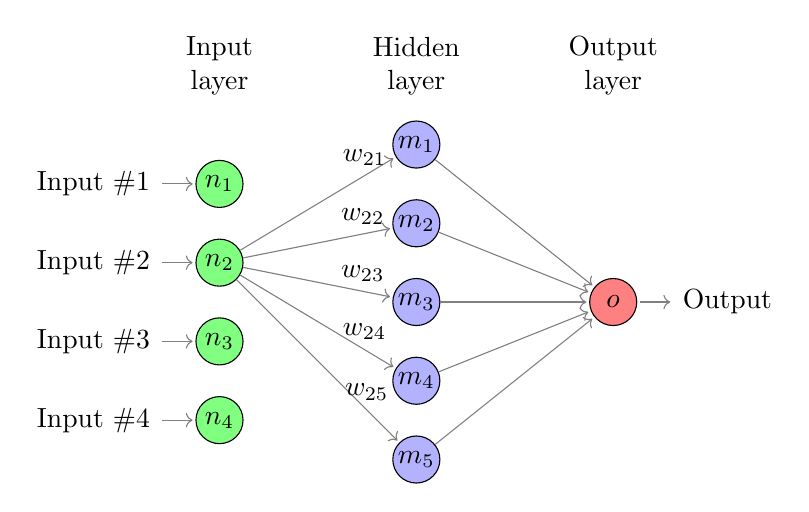
\begin{tikzpicture}[shorten >=1pt,->,draw=black!50, node distance=\layersep]
%https://tex.stackexchange.com/questions/96846/how-to-place-label-in-middle-of-line-above-and-below-with-tikz
    \tikzstyle{every pin edge}=[<-,shorten <=1pt]
    \tikzstyle{neuron}=[circle,fill=black!25,minimum size=17pt,inner sep=0pt, draw=black]
    \tikzstyle{input neuron}=[neuron, fill=green!50];
    \tikzstyle{output neuron}=[neuron, fill=red!50];
    \tikzstyle{hidden neuron}=[neuron, fill=blue!30];
    \tikzstyle{annot} = [text width=4em, text centered]

    % Draw the input layer nodes
    \foreach \name / \y in {1,...,4}
    % This is the same as writing \foreach \name / \y in {1/1,2/2,3/3,4/4}
        \node[input neuron, pin=left:Input \#\y] (I-\name) at (0,-\y) {$n_\y$};

    % Draw the hidden layer nodes
    \foreach \name / \y in {1,...,5}
        \path[yshift=0.5cm]
            node[hidden neuron] (H-\name) at (\layersep,-\y cm) {$m_\y$};

    % Draw the output layer node
    \node[output neuron,pin={[pin edge={->}]right:Output}, right of=H-3] (O) {$o$};

    % Connect every node in the input layer with every node in the
    % hidden layer.
%    \foreach \source in {1,...,4}
%        \foreach \dest in {1,...,5}
%            \draw (I-\source) -- node[below] {$w_ij$} ++ (H-\dest);


%    \foreach \source in {1,...,4}
        \foreach \dest in {1,...,5}
            \draw (I-2) -- node[above, pos=0.8] {$w_{2\dest}$} ++ (H-\dest);

    % Connect every node in the hidden layer with the output layer
    \foreach \source in {1,...,5}
        \path (H-\source) edge (O);

    % Annotate the layers
    \node[annot,above of=H-1, node distance=1cm] (hl) {Hidden layer};
    \node[annot,left of=hl] {Input layer};
    \node[annot,right of=hl] {Output layer};
\end{tikzpicture}
  \end{minipage}
  \vfill
\begin{minipage}[t][0.5\textheight][t]{\textwidth}

\end{minipage}


\end{frame}




\begin{frame}[fragile]{Point Variance of Linear Predictor}

\begin{align*}
\action<+->{ &=&&}
\\
\action<+->{  &=   && }
\end{align*}
\action<+->{The}
\end{frame}



\begin{frame}[fragile]{Correlation}
\begin{itemize}
\item[] \textbf{Serial No.} is basically uncorrelated with anything. \pause
\item[] \textbf{Admit} is highly correlated with \textbf{CGPA}, \textbf{TOEFL Score} and \textbf{GRE Score}\pause
\item[] \textbf{Research} has a lowish correlation with \textbf{Admit}, but also with everything else.  
\end{itemize}
\end{frame}











\begin{frame}[fragile]{Bias, Variance and Parameters}
  \begin{minipage}[t][0.5\textheight][t]{\textwidth}
	\centering
	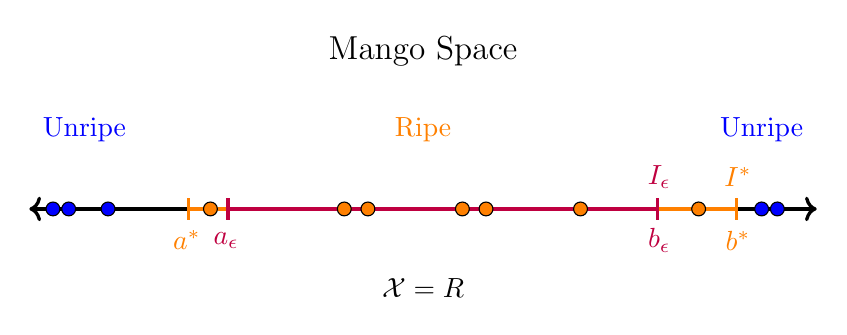
\begin{tikzpicture}
		\draw[<->,very thick] (-5,0) -- (5,0);
		\draw[color = orange, |-|,very thick] (-3,0) -- (4,0);
		\node[color=orange] at (4,.4) {$I^*$};
		\node at (0,2) {\large Mango Space} ;
		\node at (0,-1) {$\mathcal{X} = \mathbb{R}$} ;
		\node [color=blue] at (-4.3,1) {Unripe} ;
		\node [color=blue] at (4.3,1) {Unripe} ;
		\node [color=orange] at (0,1) {Ripe} ;

		\node [color=orange] at (-3,-.4) {$a^*$} ;
		\node [color=orange] at (4,-.4) {$b^*$} ;

		\draw [color=purple, |-|,very thick] (-2.5,0) -- (3,0);
		\node [color=purple] at (3,.4) {$I_\epsilon$} ;
		\node [color=purple] at (-2.5,-.4) {$a_\epsilon$} ;
		\node [color=purple] at (3,-.4) {$b_\epsilon$} ;

%		\draw [color=olive, |-|,very thick] (-3.5,0) -- (2.5,0);
%		\node [color=olive] at (3,.4) {$h_{\mathcal{T}}$} ;



		\node[circle,draw=black, fill=orange, inner sep=0pt,minimum size=5pt] at (2,0) {};
		\node[circle,draw=black, fill=orange, inner sep=0pt,minimum size=5pt] at (-1,0) {};
		\node[circle,draw=black, fill=orange, inner sep=0pt,minimum size=5pt] at (-.7,0) {};
		\node[circle,draw=black, fill=orange, inner sep=0pt,minimum size=5pt] at (.5,0) {};
		\node[circle,draw=black, fill=orange, inner sep=0pt,minimum size=5pt] at (.8,0) {};
		\node[circle,draw=black, fill=orange, inner sep=0pt,minimum size=5pt] at (-2.7,0) {};
		\node[circle,draw=black, fill=orange, inner sep=0pt,minimum size=5pt] at (3.5,0) {};

		\node[circle,draw=black, fill=blue, inner sep=0pt,minimum size=5pt] at (-4.5,0) {};
		\node[circle,draw=black, fill=blue, inner sep=0pt,minimum size=5pt] at (-4,0) {};
		\node[circle,draw=black, fill=blue, inner sep=0pt,minimum size=5pt] at (-4.7,0) {};
		\node[circle,draw=black, fill=blue, inner sep=0pt,minimum size=5pt] at (4.3,0) {};
		\node[circle,draw=black, fill=blue, inner sep=0pt,minimum size=5pt] at (4.5,0) {};
	\end{tikzpicture}
  \end{minipage}
  \vfill
  \begin{minipage}[t][0.5\textheight][t]{\textwidth}
Lets understand this visually.
$$
Err(x_0) = \sigma_\epsilon^2 + [E_\cT[\hat f(x_0)] - f(x_0)]^2 + E_\cT\big[ \hat{f}(x_0) - E_\cT[\hat{f}(x_0)] \big]^2\,.
$$\pause
Consider a data set, 
\end{minipage}
\end{frame}





























